\begin{figure*}
\centering     %%% not \center

\begin{subfigure}[h][Turtlebot3 Reward]{\label{fig:turtlebot_reward}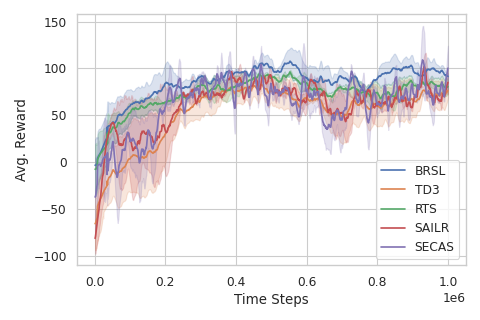
\includegraphics[scale=0.25]{Figures/Turtlebot3_reward.png}}
\end{subfigure}
\begin{subfigure}[h][Quadrotor Reward]{\label{fig:drone_reward}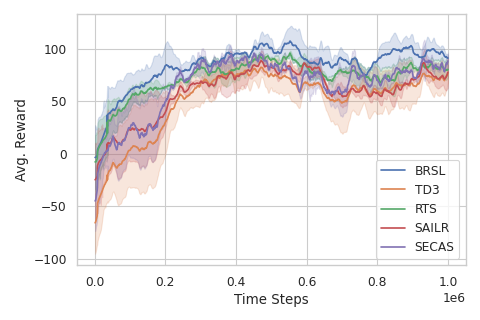
\includegraphics[scale=0.25]{Figures/Quadrotor_reward.png}}
\end{subfigure}
\begin{subfigure}[h][Point Reward]{\label{fig:point_reward}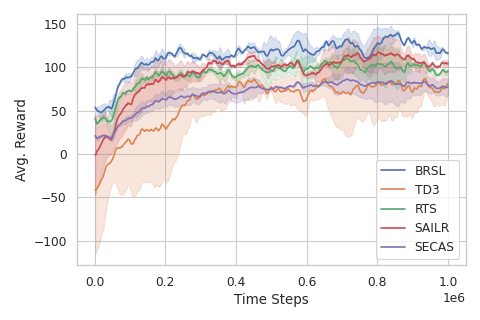
\includegraphics[scale=0.25]{Figures/Point_reward.png}}
\end{subfigure}
\begin{subfigure}[h][\tbold{Hexarotor Reward}]{\label{fig:hexarotor_reward}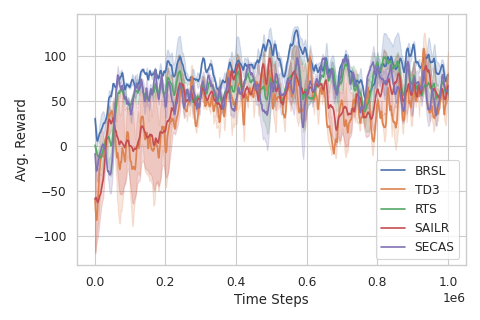
\includegraphics[scale=0.25]{Figures/Hexarotor_reward.png}}
\end{subfigure}
%\hspace{10mm}
%\subfigure[Arrival and collisions rates are in bold and dashed lines, respectively.]{\label{fig:Ng2}\includegraphics[scale=0.25]{Figures/turtlebot_safety.png}}

\caption{Average reward over time of BRSL, RTS \cite{conf:modelBasedReachRL}, SAILR \cite{wagener2021safe}, and a vanilla TD3 baseline for each of our experiments.}
\label{fig:sim_results}
\vspace{-2mm}
\end{figure*}

\begin{table*}[ht]
\caption{Goal-based experiment results (best values in bold)}
\label{tbl:comparison}
\vspace{-3mm}
\centering
\resizebox{1.98\columnwidth}{!}{\begin{tabular}{ c|c|c|c|c|c||c|c|c|c|c } 
 %\hline
 & \multicolumn{5}{c||}{Turtlebot} & \multicolumn{5}{c}{Quadrotor} \\
 & BRSL & RTS & SAILR & \tbold{SECAS}&Baseline  & BRSL & RTS & SAILR & \tbold{SECAS}& Baseline  \\
 \hline
 Goal Rate [\%] &
    \textbf{57} & 52 & 48 & \tbold{53} & 42  &
    \textbf{76} & 66 & 61 & \tbold{59} & 54 \\
 Collision Rate [\%] &
    \textbf{0.0} & \textbf{0.0} & 7.3 & \tbold{\textbf{0.0}} &48 
    &\textbf{0.0} & \textbf{0.0} & 9.2& \tbold{\textbf{0.0}} & 59\\
 Mean/Max Speed [m/s] & 
    .07 / \textbf{0.18} & 0.05 / 0.15 & .07 / 0.17 & \tbold{.06 / 0.15} &\textbf{.08} / \textbf{.18} & 
    3.6 / \textbf{7.9} &  3.3 / 7.8 & \textbf{3.7} / \textbf{7.9} & \tbold{3.2 / 7.8} & \textbf{3.7} / \textbf{7.9}\\
 Mean Reward &
    \textbf{86} & 78 & 68 & \tbold{66} & 63 &
    \textbf{82} & 73 & 61 & \tbold{68} & 57 \\
 Mean $\pm$ Std. Dev.  &
    \multirow{2}{*}{50.41 $\pm$ 20.5} & \multirow{2}{*}{100.74 $\pm$ 60.5} & \multirow{2}{*}{30.53 $\pm$ 10.8} & \tbold{\multirow{2}{*}{22.4 $\pm$ 14.66}} & \multirow{2}{*}{\textbf{10.21} $\pm$ 10.05} &
    \multirow{2}{*}{60.33 $\pm$ 20.34} & \multirow{2}{*}{260.85 $\pm$ 140.67} & \multirow{2}{*}{45.31 $\pm$ 20.84} & \tbold{\multirow{2}{*}{39.7 $\pm$ 34.08}} & \multirow{2}{*}{\textbf{20.63} $\pm$ 30.2} \\
    Compute Time [ms] &&&&&&& &&\\
 \hline
    \end{tabular}}
\vspace{-2mm}
\end{table*}

\begin{table*}[ht]
    \caption{Path Following Results (best values in bold)}
    \label{tbl:point_robot}
    \vspace{-2mm}
    \centering
    \resizebox{1.98\columnwidth}{!}{\begin{tabular}{ c|c|c|c|c|c||c|c|c|c|c|c}
    & \multicolumn{5}{c||}{Point Environment} & \multicolumn{5}{c}{\tbold{Hexarotor}} \\
         & BRSL & RTS & SAILR &\tbold{SECAS} &Baseline & \tbold{BRSL} & \tbold{RTS} & \tbold{SAILR} &\tbold{SECAS} &\tbold{Baseline}\\
         \hline
         Collisions [\%] &
            \textbf{0.0} & \textbf{0.0} & 4.9 & \tbold{\textbf{0.0}} &11.4 & \tbold{\textbf{0.0}} & \tbold{2} & \tbold{14} & \tbold{7} & \tbold{63} \\
         Mean Speed [m/s] & 
            0.76 & 0.72 & 0.78 & \tbold{0.68} &\textbf{0.86} & \tbold{3.81} & \tbold{3.4} & \tbold{3.84} & \tbold{3.1} & \tbold{\textbf{3.94}} \\
         Max Speed [m/s] & 
            \textbf{2.00} & 1.89 & \textbf{2.00} & \tbold{1.74} &\textbf{2.00} & \tbold{8.4} & \tbold{8.1} & \tbold{8.2} & \tbold{7.95} & \tbold{\textbf{8.7}} \\
         Mean Reward &
            \textbf{118} & 93 & 88 & \tbold{78} &73 & \tbold{\textbf{84}} & \tbold{78} & \tbold{69} & \tbold{62} & \tbold{57}\\
         Compute Time [ms] &
            30.0 $\pm$ 10.2 & 60.18 $\pm$ 20.09 & 20.49 $\pm$ 10.34 & \tbold{16.42 $\pm$ 8.7} &\textbf{8.64} $\pm$ 1.14 & \tbold{71.93 $\pm$ 34.52} & \tbold{290.96 $\pm$ 157.24} & \tbold{67.86 $\pm$ 22.34} & \tbold{48.53 $\pm$ 28.69} & \tbold{\textbf{32.79 $\pm$ 27.6}} \\
         \hline
    \end{tabular}}
\vspace{-2mm}
\end{table*}


\section{Evaluation} \label{sec:eval}

%\subsection{Safe Robot Navigation to a Goal}
We evaluate BRSL on two types of environments: safe navigation to a goal (a Turtlebot in Gazebo and a quadrotor platform in Unreal Engine $4$), and path following (a point mass based on \cite{achiam2017constrained,wagener2021safe} and a hexarotor in wind in Unreal Engine $4$).
Figure \ref{fig:sim_envs} shows example environments.
%To test the robustness of BRSL, we subject the hexarotor to uncertain wind, which violates Assumption \ref{assumption:stop}, to test the robustness of BRSL.
All code is run on a desktop computer with an Intel i5 11600 CPU and a RTX 3060 GPU. 
%\footnote{We plan to make the code open-source after publication.}.
Our code is available \href{https://github.com/Mahmoud-Selim/Safe-Reinforcement-Learning-for-Black-Box-Systems-Using-Reachability-Analysis}{\underline{\color{blue}{online}}}.
We aim to assess the following:
(a) How does BRSL compare against other safe RL methods (RTS \cite{conf:modelBasedReachRL}, SAILR \cite{wagener2021safe}, and SECAS \cite{dalal2018safe})?
(b) How conservative is BRSL?
(c) Can BRSL run in real time?
% \begin{itemize}
%     \item How does BRSL compare against a vanilla baseline (unsafe) RL agent and other safe RL methods (RTS \cite{conf:modelBasedReachRL}, SAILR \cite{wagener2021safe}, \tbold{and (SECAS) \cite{dalal2018safe}}) in terms of reward and safety?
%     \item How conservative is BRSL in environments where high reward states are near unsafe regions?
%     \item Can BRSL be implemented in real time for safety-critical systems?
% \end{itemize}

% \subsection{Setup}
\textbf{Setup.}
We use TD3 \cite{conf:TD3} as our RL agent, after determining empirically that it outperforms SAC \cite{conf:SAC} and DDPG \cite{conf:DDPG}. %(we justify this choice in the supplementary section).
We randomly initialize the policy.
Since the agent outputs continuous actions, to aid the exploration process, we inject zero-mean Gaussian noise with a variance of $0.5$ that is dampened each time step.
Note that this does not affect safety since our safety layer adjusts the output of the RL agent.

For each robot, to perform reachability analysis with Algorithm \ref{alg:LipReachability}, we collect $500$ time steps of noisy state/input data (as per \eqref{eq:data}) offline in an empty environment while applying random control inputs.
We found this quantity of data sufficient to ensure safety empirically; we leave a formal analysis of the minimum amount of data for future work.

We parameterize the environment \tbold{model} as an ensemble of neural networks, each modeling a Gaussian distribution over future states and observations.
Each network has $4$ layers, with hidden layers of size 200, and leaky ReLU activations with a negative slope of $0.01$.
We use a stochastic model wherein the ensemble predicts the parameters of a probability distribution, which is sampled to produce a state as in \cite{chua2018deep}.


% \subsubsection{Goal-Based Environments
\textit{Goal-Based Environments.}
The Turtlebot 3 and the quadrotor seek to navigate to a random circular goal region $\statespace\goal \subset \statespace$ while avoiding randomly-generated obstacles $\statespace\obs \subset \statespace$. %, as shown in Fig.~\ref{fig:turtleee} for the Turtlebot and Fig.~\ref{fig:droneee} for the quadrotor.
% Both Turtlebot's and the quadrotor's goals are randomly selected at the beginning of each episode.
Each robot starts in a safe location at the center of the map.
Each task is episodic, ending if the robot reaches the goal, crashes, or exceeds a time limit.
Both robots have uncertain, noisy dynamics as in \eqref{eq:sys}.
We discretize time at $10$ Hz.

The Turtlebot's control inputs are longitudinal velocity in $[0.00,0.25]$ m/s and angular velocity in $[-0.5, 0.5]$ rad/s (these are the bounds of $\actionspace_k$).
The robot has wheel encoders, plus a planar lidar that generates $18$ range measurements evenly spaced in a $180^\circ$ arc in front of the robot.
The robot requires $\nbrk = 6$ time steps to stop, so we set $\nplan = 8$.

The quadrotor control inputs are commanded velocities up to 5 m/s in each spatial direction at each time step.
\tb{We note that we also experimented with learning low-level rotor speeds versus high-level velocity commands, and found that the velocity commands created the fairest testing conditions across all agents}. The robot is equipped with an IMU and a 16-channel lidar which receives range measurements around the robot in a $50^\circ$ vertical arc and a $360^\circ$ horizontal arc.
The robot has $\nbrk = 10$, so we set $\nplan = 11$.

%We use the following reward for goal-based environments:
%\newcommand{\indic}{\mathbb{I}}
%\begin{align}\begin{split}
%    \rewfunc(\RLstate_k,\RLaction_k) =
%    &+10^3\cdot \indic\left(\vcstate_k \in X\goal\right) +\\
%    &-20\cdot d\left(\vcstate_k,\statespace\goal\right)+ \\
%    &-10^3\cdot\indic\left(\RLaction_k\ \text{is unsafe}\right), %\end{split}
%\end{align} 
%where $\indic(\cdot)$ returns 1 if its argument is true or 0 otherwise, $d(\cdot,X\goal)$ returns the Euclidean distance to the center of the goal region, and the safety of $\RLaction_k$ is checked using the reachable set of the RL agent's plan (before adjustment).
%The robot position is estimated from the odometry of the robot.


%\TODO{These robot-specific details should be moved to the supplement.}



% \subsection{Choosing an RL Agent}
%\TODO{This subsection can be moved to the supplement; in this section, we just need to say we're using TD3.}
%We chose TD3 \cite{conf:TD3} as our RL agent. %(we justify this choice in the supplementary section).
%Since the agent outputs continuous actions, to aid the exploration process, we inject zero-mean Gaussian noise with a variance of $0.5$ that is dampened by a factor of $0.99995$ per time step.




% \begin{figure*}[ht]
% \vspace{-0.05cm}
%     \centering
%     % \begin{tabular}{ p{0.330\textwidth}  p{0.330\textwidth} p{0.330\textwidth}}
%     % \resizebox{0.32\textwidth}{!}{
%             \begin{subfigure}[h]{0.33\textwidth}
%      \centering
%         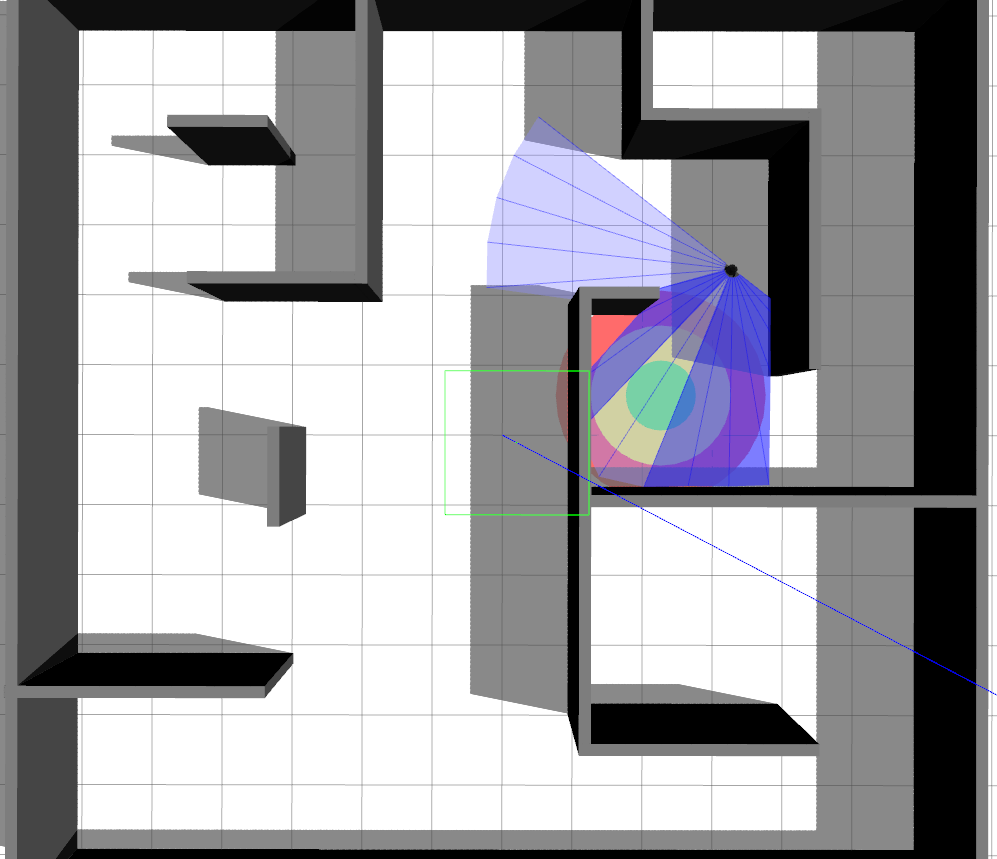
\includegraphics[scale=0.11]{Figures/turtleee.png}
%         \caption{Turtlebot Environment. The goal for the robot (black dot) is to reach the green circle.}%It is designed so that unsafe RL experience many collisions.} %%The goal is the green circle. Its position is also changed at each episode}
%         \label{fig:turtleee}
%     \end{subfigure}
%     %   } 
% %   &
% %   \resizebox{0.32\textwidth}{!}{
%             \begin{subfigure}[h]{0.33\textwidth}
%      \centering
%         \includegraphics[scale=0.33]{Figures/turtlebot_reward.png}
%         \caption{Turtlebot reward comparisons.}% Both safe agents learn to achieve higher reward than the unsafe TD3}
%         \label{fig:safe_agent}
%     \end{subfigure}
%     %  }
%     %     &
% %   \resizebox{0.32\textwidth}{!}{
%             \begin{subfigure}[h]{0.33\textwidth}
%      \centering
%         \includegraphics[scale=0.32]{Figures/turtlebot_safety.png}
%         \caption{Arrival and collisions rates are in bold and dashed lines, respectively.} %Both BRSL and RTS have no collisions and baseline TD3 learns to avoid obstacles. All three agents learn to arrive at goals with time.
%         \label{fig:img_with_vars}
%     \end{subfigure}
% %      }
% %  \end{tabular}
% \caption{Comparison between TD3, BRSL, and RTS in the Turtlebot navigation.}
%     \label{fig:turtleee3fig}%\vspace{-4mm}
%     \vspace{-4mm}
% \end{figure*}

% \subsubsection{Path Following Environments}
\textit{Path Following Environments.}
These experiments assess BRSL's conservativeness is by placing the highest reward adjacent to obstacles.

The goal for the point robot is to follow a circular path of radius $r$ as quickly as possible while constrained to a region smaller than the target circle.
The point robot is a 2-D double integrator with position and velocity as its state: $\vcstate_k = (x_k,y_k,\dot{x}_k,\dot{y}_k)$.
It has a maximum velocity of 2 m/s, and its control input is acceleration up to 1 m/s$^2$ in any direction.
We use these dynamics as in \cite{achiam2017constrained,wagener2021safe} to enable a fair test against other methods that require a robot model.
We define a box-shaped safe set (the complement of the obstacle set) as $\statespace\safe = \{\vcstate_k \in \statespace : |x_k| \le x_{\max},  |y_k| \le y_{\max}\}$, with $\norm{(x_{\max}, y_{\max})}_2 < r$.
We use a reward that encourages traveling quickly near the unsafe set: $\rewfunc (\RLstate_k,\RLaction_k) = \frac{(\dot{x}_k, \dot{y}_k) \cdot (-y_k, x_k)}{1 + \big| \norm{(x_k, y_k)}_2 - r\big|}$.
% \begin{align}\begin{split}
%     \rewfunc (\RLstate_k,\RLaction_k) = \frac{(\dot{x}_k, \dot{y}_k) \cdot (-y_k, x_k)}{1 + \big| \norm{(x_k, y_k)}_2 - r\big|}.
% \end{split}\end{align}

The hexarotor has the same setup as the quadrotor, but with the addition of wind as an external disturbance.
The goal of the hexarotor is to pass through $10$ checkpoints in a fixed order while subject to wind (constant speed and direction) and randomly-placed obstacles.
Note, offline data collection was performed under wind conditions.
% As for the robot's action, it's a vector containing the horizontal and vertical accelerations of the robot. That is $\RLaction \in \mathbbm{R}^2 = (a_x, a_y)$.
%\TODO{explain what the control inputs and observations are for the point robot}


%\begin{figure}[t]
%\centering     %%% not \center
%\subfigure[Turtlebot Environment.]{\label{fig:turtlebo_env}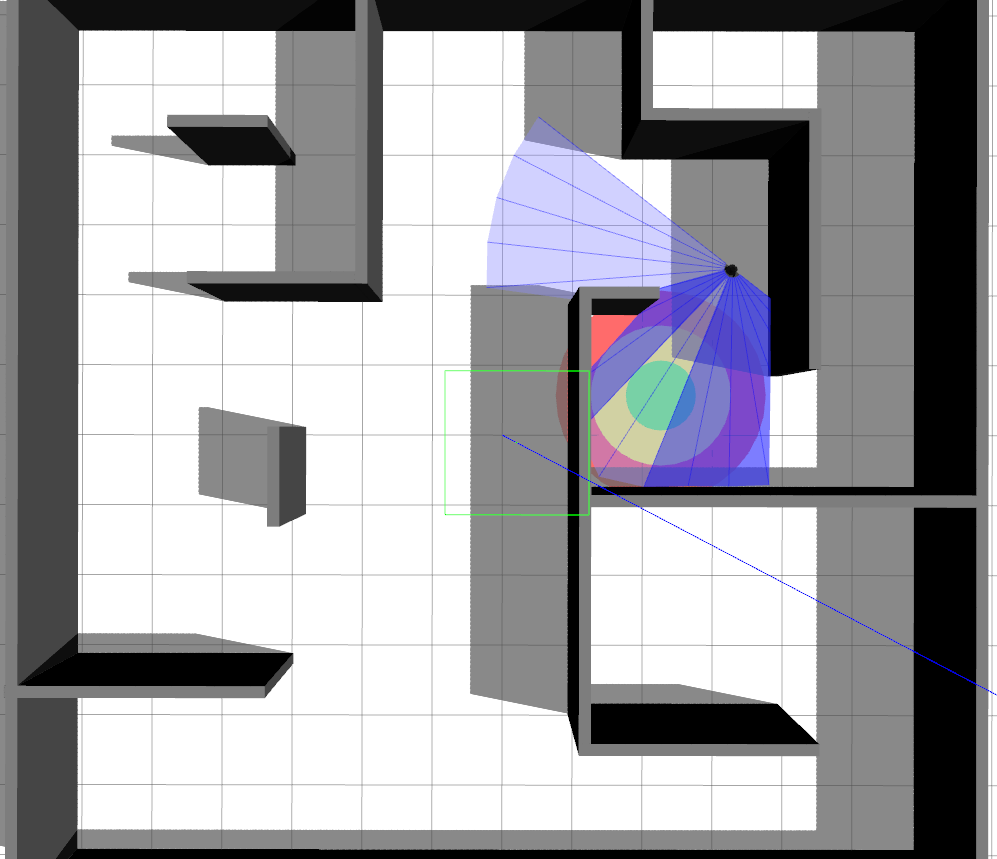
\includegraphics[scale=0.13]{Figures/turtleee.png}}
%\hspace{10mm}
%\subfigure[Turtlebot reward comparisons.]{\label{fig:turtlebot_reward}\includegraphics[scale=0.4]{Figures/turtlebot_reward.png}}
%\hspace{10mm}
%\subfigure[Arrival and collisions rates are in bold and dashed lines, respectively.]{\label{fig:Ng2}\includegraphics[scale=0.25]{Figures/turtlebot_safety.png}}
%\caption{Comparison between TD3, BRSL, and RTS in the Turtlebot navigation.}
%\label{fig:turtleee3fig}
%\end{figure}

% \begin{figure*}[!htbp]
% \vspace{-0.05cm}
%     \centering
%     % \begin{tabular}{ p{0.330\textwidth}  p{0.330\textwidth} p{0.330\textwidth}}
%     % \resizebox{0.32\textwidth}{!}{
%             \begin{subfigure}[h]{0.33\textwidth}
%      \centering
%         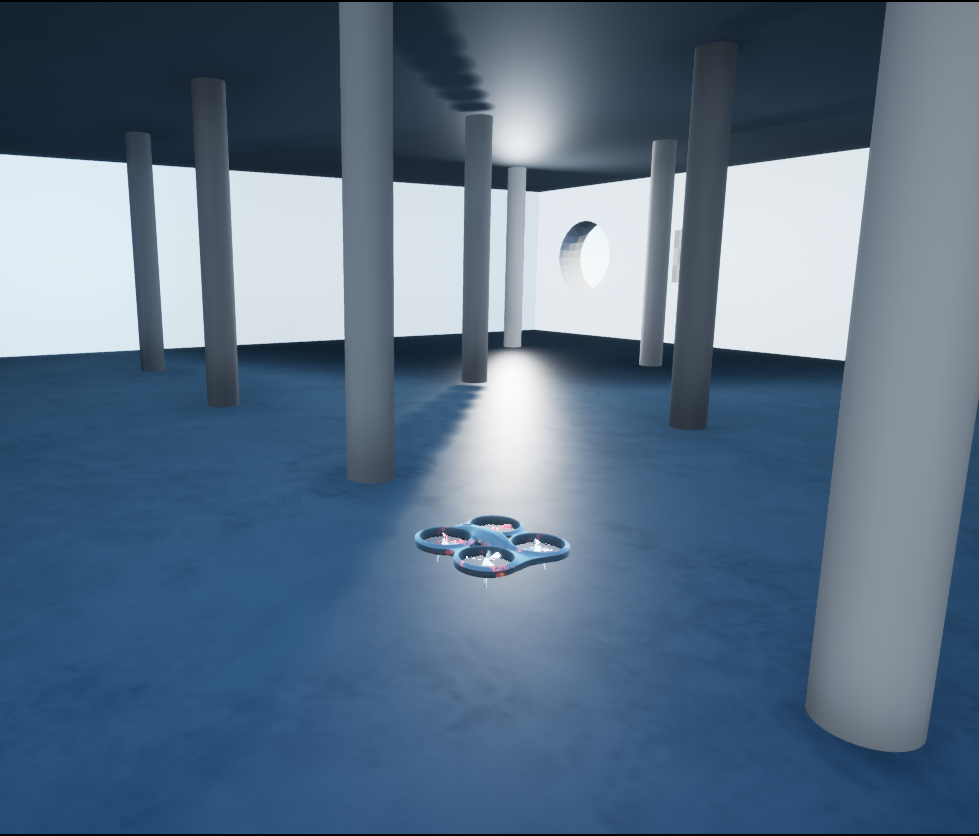
\includegraphics[scale=0.11]{Figures/droneee.png}
%         \caption{quadrotor Environment.
%         The goal is the circular hole in the wall.}
%         \label{fig:droneee}
%     \end{subfigure}
% %       } 
% %   &
% %   \resizebox{0.32\textwidth}{!}{
%             \begin{subfigure}[h]{0.33\textwidth}
%      \centering
%         \includegraphics[scale=0.33]{Figures/drone_reward.png}
%         \caption{quadrotor reward comparisons.}% Both safe agents learn to achieve higher reward than the unsafe TD3}
%         \label{fig:drone_reward}
%     \end{subfigure}
%     %  }
%     %     &
% %   \resizebox{0.32\textwidth}{!}{
%             \begin{subfigure}[h]{0.33\textwidth}
%      \centering
%         \includegraphics[scale=0.32]{Figures/drone_safety.png}
%         \caption{Arrival and collisions rates are in bold and dashed lines, respectively.}%. Both BRSL and RTS have no collisions and baseline TD3 learns to avoid obstacles. All three agents learn to arrive at goals with time.}
%         \label{fig:drone_safety}
%     \end{subfigure}
% %      }
% %  \end{tabular}
% \caption{Comparison between TD3, BRSL, and RTS in the quadrotor experiment.}
%     \label{fig:droneee3fig}%\vspace{-4mm}
%     \label{fig:drone_fig}
%     \vspace{-4mm}
% \end{figure*}

%\begin{figure}
%\centering     %%% not \center
%\subfigure[quadrotor Environment.]{\label{fig:drone_env}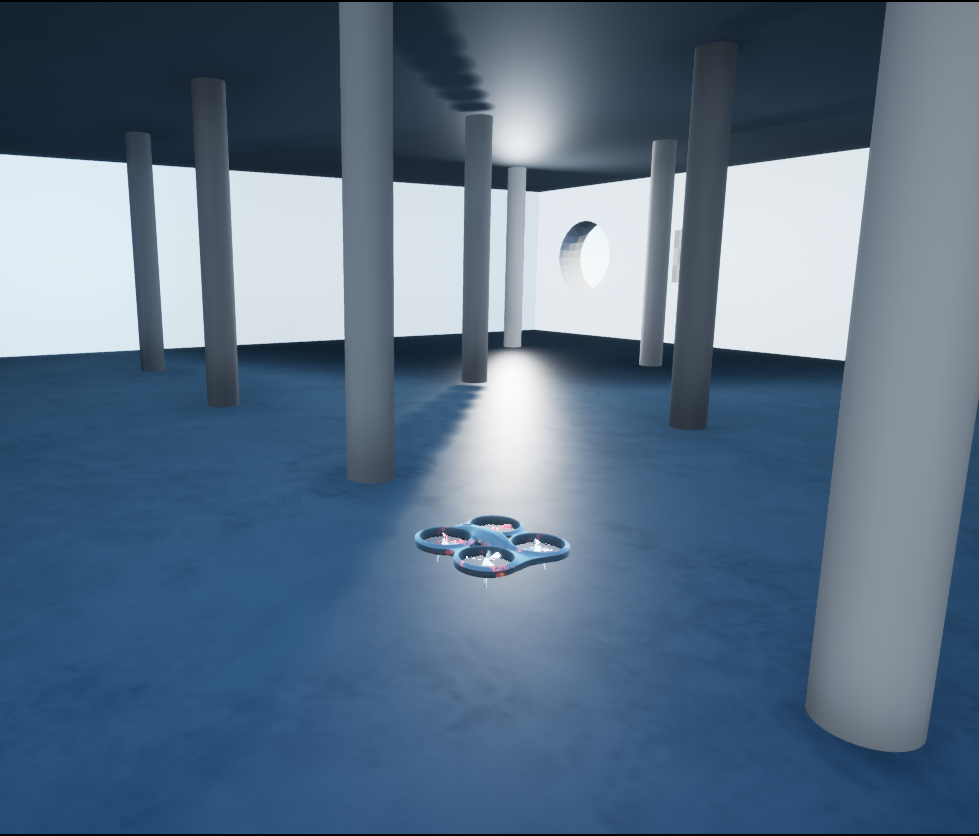
\includegraphics[scale=0.135]{Figures/droneee.png}}
%\hspace{10mm}
%\subfigure[quadrotor reward comparisons.]{\label{fig:drone_reward}\includegraphics[sca%le=0.4]{Figures/drone_reward.png}}
%\hspace{10mm}
%\subfigure[Arrival and collisions rates are in bold and dashed lines, respectively.]{\label{fig:Ng2}\includegraphics[scale=0.25]{Figures/turtlebot_safety.png}}
%\caption{Comparison between TD3, BRSL, and RTS in the %quadrotor experiment.}
%\label{fig:drone_fig}
%\end{figure}



% \subsection{Results and Discussion}
\textbf{Results and Discussion.}
\tb{The results are summarized in Tables \ref{tbl:comparison} and \ref{tbl:point_robot}, and in Figure \ref{fig:sim_results}.
%RTS is almost the same in terms of reward and arrival rate as our BRSL framework.
BRSL outperforms the other methods in terms of reward and safety, is not overly conservative, and can operate in real time, despite lacking a model of the robot \emph{a priori}.
While SAILR and the baseline RL agent achieved higher speeds, both experienced collisions, unlike BRSL, RTS, and SECAS.
In contrast to RTS, which chooses from a low-dimensional parameterized plans, BRSL outputs a more flexible sequence of actions.
Furthermore RTS' planning time increases with state space dimension due to computing a halfspace representation of reachable set zonotopes, which grows exponentially in the number of generators \cite{althoffphdthesis}.
BRSL avoids this computation by using \eqref{prog:collision_check}.
Instead, the quantity of data for BRSL determines the computation time of $\vc{M}_j$ from Algorithm \ref{alg:LipReachability}, used for reachability and adjusting unsafe actions.
Therefore, one can ensure the amount of data allows real time operation; choosing the data optimally is left to future work.
Finally, BRSL uses zonotopes to exactly represent safety constraints, whereas SECAS uses a more conservative first-order approximation.
This results in BRSL achieving higher reward with slightly slower computation time (but still fast enough for real time operation).}
% It is possible RTS can be more efficient with hyperparameter tuning; our focus is BRSL's real-time capability.

% \tb{
% We explain BRSL's performance advantages as follows.
% First, BRSL outputs a more flexible sequence of actions than RTS, which chooses from a low-dimensional parameterized set of plans.
% % Second, SAILR does not enforce hard safety constraints, unlike BRSL.
% Second, BRSL exactly represents safety constraints, whereas SECAS uses a more conservative first-order approximation.
% }
% \begin{table}[ht]
%     \caption{Mean $\pm$ std. dev. of computation time in seconds.}
%     \label{tab:runtimes}
%     \centering
%     \begin{tabular}{c | c | c | c | c }
%          Robot& BRSL & RTS & SAILR & Baseline \\
%          \hline
%          Turtlebot3 & 0.05 $\pm$ 0.02 & 0.10 $\pm$ 0.06 & 0.03 $\pm$ 0.01 & 0.01 $\pm$ 0.01 \\
%          Quadrotor & 6 $\pm$ 2 & 26 $\pm$ 14 & 4.5 $\pm$ 2 & 2 $\pm$ .3 \\
%          %Hexarotor (12/6) & x $\pm$ y & x $\pm$ y & x $\pm$ y & x $\pm$ y \\
%          Point & 3 $\pm$ 1 & 6 $\pm$ 2 & 2 $\pm$ 1 & .8 $\pm$ .07 \\
%          \hline
%     \end{tabular}
% \end{table}

